\section{Theorie}
\label{sec:Theorie}
Als $LC$-Kette wird eine Kette aus $LC$-Schwingkreisen bezeichnet.
Ein $LC$-Schwingkreis besteht dabei aus einer Induktivität $L$ und einer Kapazität $C$. Je nachdem, wie diese Bauteile
im Schwingkreis positioniert sind, wirkt eine $LC$-Schaltung als Hochpass (hohe Frequenzen passieren nahezu ungehindert die Schaltung)
oder als Tiefpass (niedrige Frequenzen können die Schaltung passieren).
\begin{figure}
    \centering
    \begin{subfigure}{0.48\textwidth}
        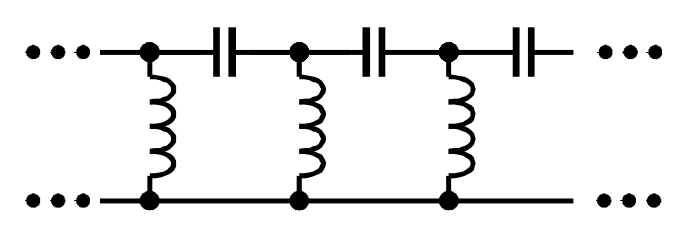
\includegraphics[width=\textwidth]{Bilder/hochpass_schema.png}
        \caption{Prinzipieller Aufbau eines Hochpass.}
        \label{fig:hoch}
    \end{subfigure}
    \begin{subfigure}{0.48\textwidth}
        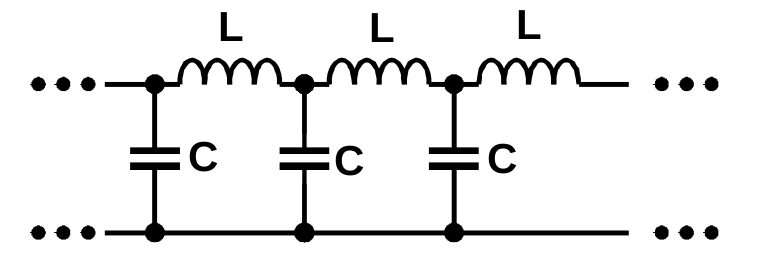
\includegraphics[width=\textwidth]{Bilder/tiefpass_schema.png}
        \caption{Prinzipieller Aufbau eines Tiefpass.}
        \label{fig:tief}
    \end{subfigure}
    \caption{Verschiedene Filterschaltungen aus Induktivitäten und Kapazitäten. \cite{Anleitung}}\label{fig:filter}
\end{figure}
In Abbildung \ref{fig:hoch} ist die notwendige Anordnung von Induktivitäten
und Kondensatoren für einen Hochpass und entsprechend für einen Tiefpass in Abbildung \ref{fig:tief} dargestellt.
Wie in Abbildung \ref{fig:tief} zu erkennen, haben zwei benachbarte Maschen eine gemeinsame Kapazität. Daher kann die $LC$-Kette analog zur
Mechanik als System gekoppelter Schwinger betrachtet werden.
Zudem kann die $LC$-Kette, für den Grenzübergang dass die Anzahl der $LC$-Kettenglieder bei endlicher Kettenlänge gegen unendlich strebt als verlustfreie Leitung betrachtet werden.

\subsection{Dispersion und Dispersionsrelation}
\label{subsec-dispersion}
Als Dispersion wird die Abhängigkeit einer Größe von der Frequenz bezeichnet.
Im vorliegenden Fall lässt sich für den n-ten Knoten der $LC$-Kette mit den Kirchhoffschen Regeln die Schwingungsgleichung herleiten.
Die Schwingungsgleichung lässt sich lösen mit einem Ansatz der Form
\begin{equation}
\centering
U(n,t)=U_{\mathrm{0}} \cdot exp(i\cdot( \omega t- n\theta )).
\label{eqn:e-ansatz}
\end{equation}
Es wird also angenommen, dass alle Maschen der $LC$-Kette mit der gleichen Frequenz $\omega$ schwingen, die Schwingung allerdings beim Durchgang durch jedes Schaltungsglied um die Phase $\sigma$ verschoben wird.
Durch Einsetzen von \eqref{eqn:e-ansatz} in die Schwingungsgleichung ergibt sich die Frequenzabhängigkeit der Phasenverschiebung zu
\begin{equation}
\centering
\omega^2=\frac{2}{LC}(1-cos{\theta}).
\label{eqn:dispersion}
\end{equation}
Aus dieser sogenannten Dispersionsrelation ist ersichtlich, dass die Frequenz \omega nicht beliebige Werte annehmen kann,
sondern auf einem endlichen Intervall definiert ist.
Es ergibt sich $0<=\omega<\frac{\sqrt{2}}{\sqrt{LC}}$.
Die Grenzfrequenz ist somit $\omega_{\mathrm{G}}=\sqrt{\frac{2}{LC}}$.
Wird die Schaltung nun etwas verallgemeinert, indem alternierend Kondensatoren zweier verschiedener Kapazitäten verwendet werden,
ergibt sich wiederum unter Verwendung der Kirchhoffschen Regeln und unter der Annahmne, das nun jeder zweite Schwingkreis mit der gleichen Amplitude
schwingt, die Dispersionsrelation
\begin{equation}
  \centering
 \omega_{1,2}^2=\frac{1}{L}\left ( \frac{1}{C_{\mathrm{1}}}+\frac{1}{C_{\mathrm{2}}} \right ) \pm \frac{1}{L} \cdot \sqrt{\left ( \frac{1}{C_{\mathrm{1}}}+\frac{1}{C_{\mathrm{2}}} \right )^2-\frac{\left(2\cdot sin(\theta)\right)^2}{C_{\mathrm{1}}C_{\mathrm{2}}}}
  \label{eqn:dispersion2}
\end{equation}
\begin{figure}
    \centering
    \includegraphics[width=0.8\textwidth]{Bilder/Dispersionäste.png}
    \caption{Dispersionskurve für eine $LC_{\mathrm{1}}C_{\mathrm{2}}$-Kette mit den auseinanderfallenden Kurvenästen. \cite{Anleitung}}
    \label{fig:dispersionskurve}
\end{figure}
Aufgrund des alternierenden Vorzeichens teilt sich die Dispersionskurve wie in Abbildung \ref{fig:dispersionskurve} zu sehen, in zwei Äste.
In der Kristallphysik wird der untere Ast als akustischer und der obere Ast als optischer Ast bezeichnet.
Es existiert also ein endlicher Frequenzbereich zwischen den Kurvenästen, indem keine Schwingungen angeregt werden können.

\subsection{Ausbreitungsgeschwindigkeit von Wellen in LC-Ketten}
Die Phasengeschwindigkeit wird definiert als des Quotienten der Wellenlänge zur Periodendauer, also der Geschwindigkeit einer bestimmten Phase.
Nach Gleichung \eqref{eqn:e-ansatz} ergibt sich unter Verwendung der Dispersionsrelation  \eqref{eqn:dispersion2}
\begin{equation}
\centering
\label{eqn:v-phase}
v_{\mathrm{Ph}}=\frac{ \Delta n}{ \Delta t}=\frac{\omega}{\theta}=\frac{\omega}{arccos(1-\frac{1}{2}\omega^2LC)}.
\end{equation}
$v_{\mathrm{Ph}}$ ist also zeitlich und räumlich unbeschränkt. Die Phasengeschwindigkeit kann also größer als die Lichtgeschwindigkeit sein und ist damit nicht zur Signalübertragung geeignet.
Zur Signalübertragung wird ein Wellenpaket benötigt.
Die Geschwindigkeit mit welcher ein Signal auf einer LC-Kette weitergeleitet wird, heißt Gruppengeschwindigkeit.
Die Gruppengeschwindigkeit bezeichnet dabei die Geschwindigkeit des Maximums der Einhüllenden des Wellenpakets.
Für unterschiedliche Phasengeschwindigkeiten kann also das Wellenpaket zerfließen.
Wie bereits in Abschnitt \ref{subsec-dispersion} erwähnt, ist $\omega$ auf einem endlichen Intervall definiert.
Für Frequenzen $\omega>=\frac{2}{\sqrt{LC}}$ würde die Gruppengeschwindigkeit imaginär werden und folglich kein Signal übertragen werden können.
\subsection{Wellenwiderstand der unendlichen Kette}
Als Eingangswiderstand der $LC$-Kette wird der Quotient aus der Spannung $U_{\mathrm{0}}$ am 1. Kondensator der Kette mit der Kapazität $\frac{C}{2}$ und dem Strom $I_{\mathrm{0}}$ welcher in die Schaltung fließt, definiert.
Mit den Kirchhoffschen Regeln und der bereits gefundenen Dispersionsrelation lässt sich der Eingangswiderstand $Z$ der $LC$-Kette berechnen.
Der Eingangswiderstand wird auch als Wellenwiderstand der $LC$-Kette bezeichnet und ergibt sich zu:
\begin{equation}
\centering
\label{eqn:wellenwiderstand}
Z(\omega)=\frac{U_{\mathrm{0}}}{I_{\mathrm{0}}}=\sqrt{\frac{L}{C}}\cdot \frac{1}{\sqrt{1-\frac{1}{4}\omega^2LC}}.
\end{equation}
Trotz der imaginären Impedanzen ist $Z(\omega)$ also reell.
Für Frequenzen $\omega<<\omega_{\mathrm{G}}$ ist also $Z(\omega)$ nahezu konstant $\sqrt{\frac{L}{C}}$.\\
Die Frequenzabhängigkeit des Wellenwiderstands ist in Abbildung \ref{fig:impedanz} dargestellt.
\begin{figure}
    \centering
\includegraphics[width=0.8\textwidth]{Bilder/frequenzabhäng_d_impedanz.png}
    \caption{Frequenzabhängigkeit des Wellenwiderstands der unendlichen Kette. \cite{Anleitung}}
    \label{fig:impedanz}
\end{figure}
Zudem ist $Z(\omega)$ nicht abhängig von der Anzahl der Kettenglieder. Eine unendliche $LC$-Kette lässt sich also simulieren, indem eine $LC$-Kette mit endlicher Anzahl an Kettengliedern mit einem nach Gleichung \eqref{eqn:wellenwiderstand} berechneten Widerstand abgeschlossen wird.

\subsection{Endlich lange $LC$-Kette}
Wenn die $LC$-Kette also mit einem Widerstand $R$ welcher dem Wellenwiderstand $Z$ entspricht, abgeschlossen wird, zeigt sich keine
Reflektion der Spannungswelle am Kettenende.
Für andere Abschlusswiderstände $R$ findet eine Reflektion am Kettenende statt.
Das Verhältnis der reflektierten Spannung $U_{\mathrm{r}}$ zur Eingangsspannung $U$ macht also Aussagen über die Art der Reflektion am Kettenende und ergibt sich zu
\begin{equation}
\centering
\label{eqn:abschluss}
\frac{U_{\mathrm{r}}}{U}=\frac{R-Z}{R+Z}.
\end{equation}

Für $R=0$, also einen Kurzschluss am Kettenende, gilt also $U_{\mathrm{r}}=-U$. Die Spannungswelle wird also mit dem Phasensprung $\pi$ reflektiert.
Für $R=\infty$ besitzt die Kette ein offenes Ende. Die Spannungswelle wird also ohne Phasensprung vollständig reflektiert.
Wie bereits erwähnt, findet für $R=Z$ keine Reflektion statt.
Für andere $R$ treten Teilreflexionen auf.
Für bestimmte Abschlusswiderstände $R$ lassen sich also durch Überlagerung der hinlaufenden Welle $A_{\mathrm{hin}}$und der reflektierten Welle $A_{\mathrm{ref}}$ stehende Wellen auf der $LC$-Kette beobachten.
Aus der Superposition der beiden Wellen ergibt sich, dass für $R=\infty$, bzw. für $R=0$ für
\begin{equation}
  \centering
  N_{\mathrm{max}} \theta_{\mathrm{k}}=k \pi \,\,\,\mathrm{ für }  \,\,\,k=1,2,...,N_{\mathrm{max}}
  \label{eqn:label1}
\end{equation}
eine stehende Welle ausgebildet wird.
Für $R=\infty$ tritt ein Spannungsbauch und für $R=0$ ein Spannungsknoten an den Kettenenden auf.
Zudem können stehende Wellen auftreten wenn am Anfang der $LC$-Kette ein  Spannungsbauch und am Kettenende ein Spannungsknoten, bzw. umgekehrt, vorliegen.
Die Bedingung hierfür lautet:
\begin{equation}
  \centering
  N_{\mathrm{max}} \theta_{\mathrm{l}}=l \frac{\pi}{2}  \,\,\,\mathrm{ für } \,\,\, l=0,1,3,5...,2N_{\mathrm{max}-1}.
  \label{eqn:label2}
\end{equation}
Es lassen sich also insgesamt $2N_{\mathrm{max}}$ Eigenschwingungen auf der $LC$-Kette anregen.
Die Frequenzen, bei denen die Eigenschwingungen und damit stehende Wellen ausgebildet werden, lassen sich jeweils über die Dispersionsrelation \eqref{eqn:dispersion} unter Verwendung der Gleichung \eqref{eqn:label1} beziehungsweise \eqref{eqn:label2} bestimmen.
